\section{Prototype}
\label{sec:prototype}
Here, we discuss our current prototype, challenges, and target applications.
Currently we compile a single shared object (\{envoy,service\}.so) for each side using compiler flags.
It is imperative we intercept syscalls on each side, and as such we must know which side of communication the library is running on to determine which network calls to intercept.
Our library is written in C and is approximately 800 LOC.

\subsection{\sysname Buffer}
The implementation started with named pipe as the main IPC mechanism.
However, due to its unidirectional nature and difficulty in incorporating synchronization mechanisms, we decided the named pipes will not suffice.

As a solution, we used \texttt{shm\_open(2)} to open a file descriptor associated with a region of shared memory and mapped it to the process using the \texttt{mmap} syscall. We allocated a circular buffer of size $2^{24}$ bytes in this shared region and read and write from it directly using \texttt{memcpy}. We will discuss our choice of the buffer size and how it affects the performance in later section. We allocated two such buffers to provide communication in each direction.

\subsection{Concurrency Challenges}
The Envoy process will write the outer request to the buffer and read the service response from the buffer; the service process will read the request (passed on by Envoy) and write the response, as returned by the service.
We now have a classic producer-consumer problem.

Our first attempt at the solution was semaphore.
We allocated two semaphores, each associated with one buffer, for the purpose of waiting and notifying.
However, semaphores did not provide a convenient way to guarantee exclusive access to the buffer.
This allowed for data races and caused the program to malfunction.

As an improvement, we moved to using mutexes across processes.
Each buffer has a mutex associated with it and also a condition variable.
We use these two constructs to guarantee mutual exclusion and to solve the consumer-producer problem.


\begin{table}[!ht]
    \begin{center}
        \resizebox{0.5\columnwidth}{!}{
            \begin{tabular}{ |c|c|c|}
                \hline
                \textbf{Function} & \textbf{Envoy} & \textbf{Service} \\
                \hline \hline
                connect & X &  \\ \hline
                accept &  & X \\ \hline
                write & X & X \\ \hline
                read & X & X \\ \hline
                writev & X &  \\ \hline
                readv & X &  \\ \hline
            \end{tabular}
        }
        \caption{Libc Functions Preloaded (Tiny C Webserver)}
        \label{t:libraries_cserver}
    \end{center}
\end{table}

\subsection{\sysname Network Calls}
The most challenging aspect of \sysname's design is properly intercepting and replicating the behavior of network system calls.
This aspect is especially challenging because Envoy uses unique handlers for request types (UDP, TCP, HTTP\{1,2,3\}, gRPC, Quic).
Further, the service itself may use the network stack in obtuse ways.
To make \sysname generalizable, one would truly have to intercept every network call (or possible network related).

This task is enormous.
Take for example, how services often take advantage of configurable aspects of the network stack like \textit{setsockopt}.
Setting options on a particular socket changes the behavior of accept, i/o, and more.
For example, our investigation of Flask~\cite{flask} revealed that it does not call \textit{accept} for new connections.
Thus, for \sysname to properly mirror the POSIX API to services in an agnostic way, it would have to model the entire state diagram for sockets.

For our prototype we have focused on HTTP. In our prototype, a service user would contact Envoy with an HTTP GET request.
Envoy uses \texttt{readv} and \texttt{writev} in order to read from and write to multiple file descriptors at the same time.
Our tiny C server\cite{tiny} uses low level file IO system calls (e.g. \texttt{read} and \texttt{write}).
We summarized the intercepted network syscalls in Table-\ref{t:libraries_cserver}.


\subsection{Initialization}\label{subsec:initialization}
We use the GCC feature \textit{\_\_attribute\_\_((costructor))} to tell GCC to compile our library such that before any functions are invoked we can load kmap.
The memory allocation can take a second or two depending on the size of memory allocated.
Thus, we run initialization/mapping functions for each side via the constructor, rather than on invocation.
This also helps optimize performance by not requiring runtime initialization checks on the functions.

\begin{figure}[!htb]
    \begin{minipage}{0.5\textwidth}
        \centering
        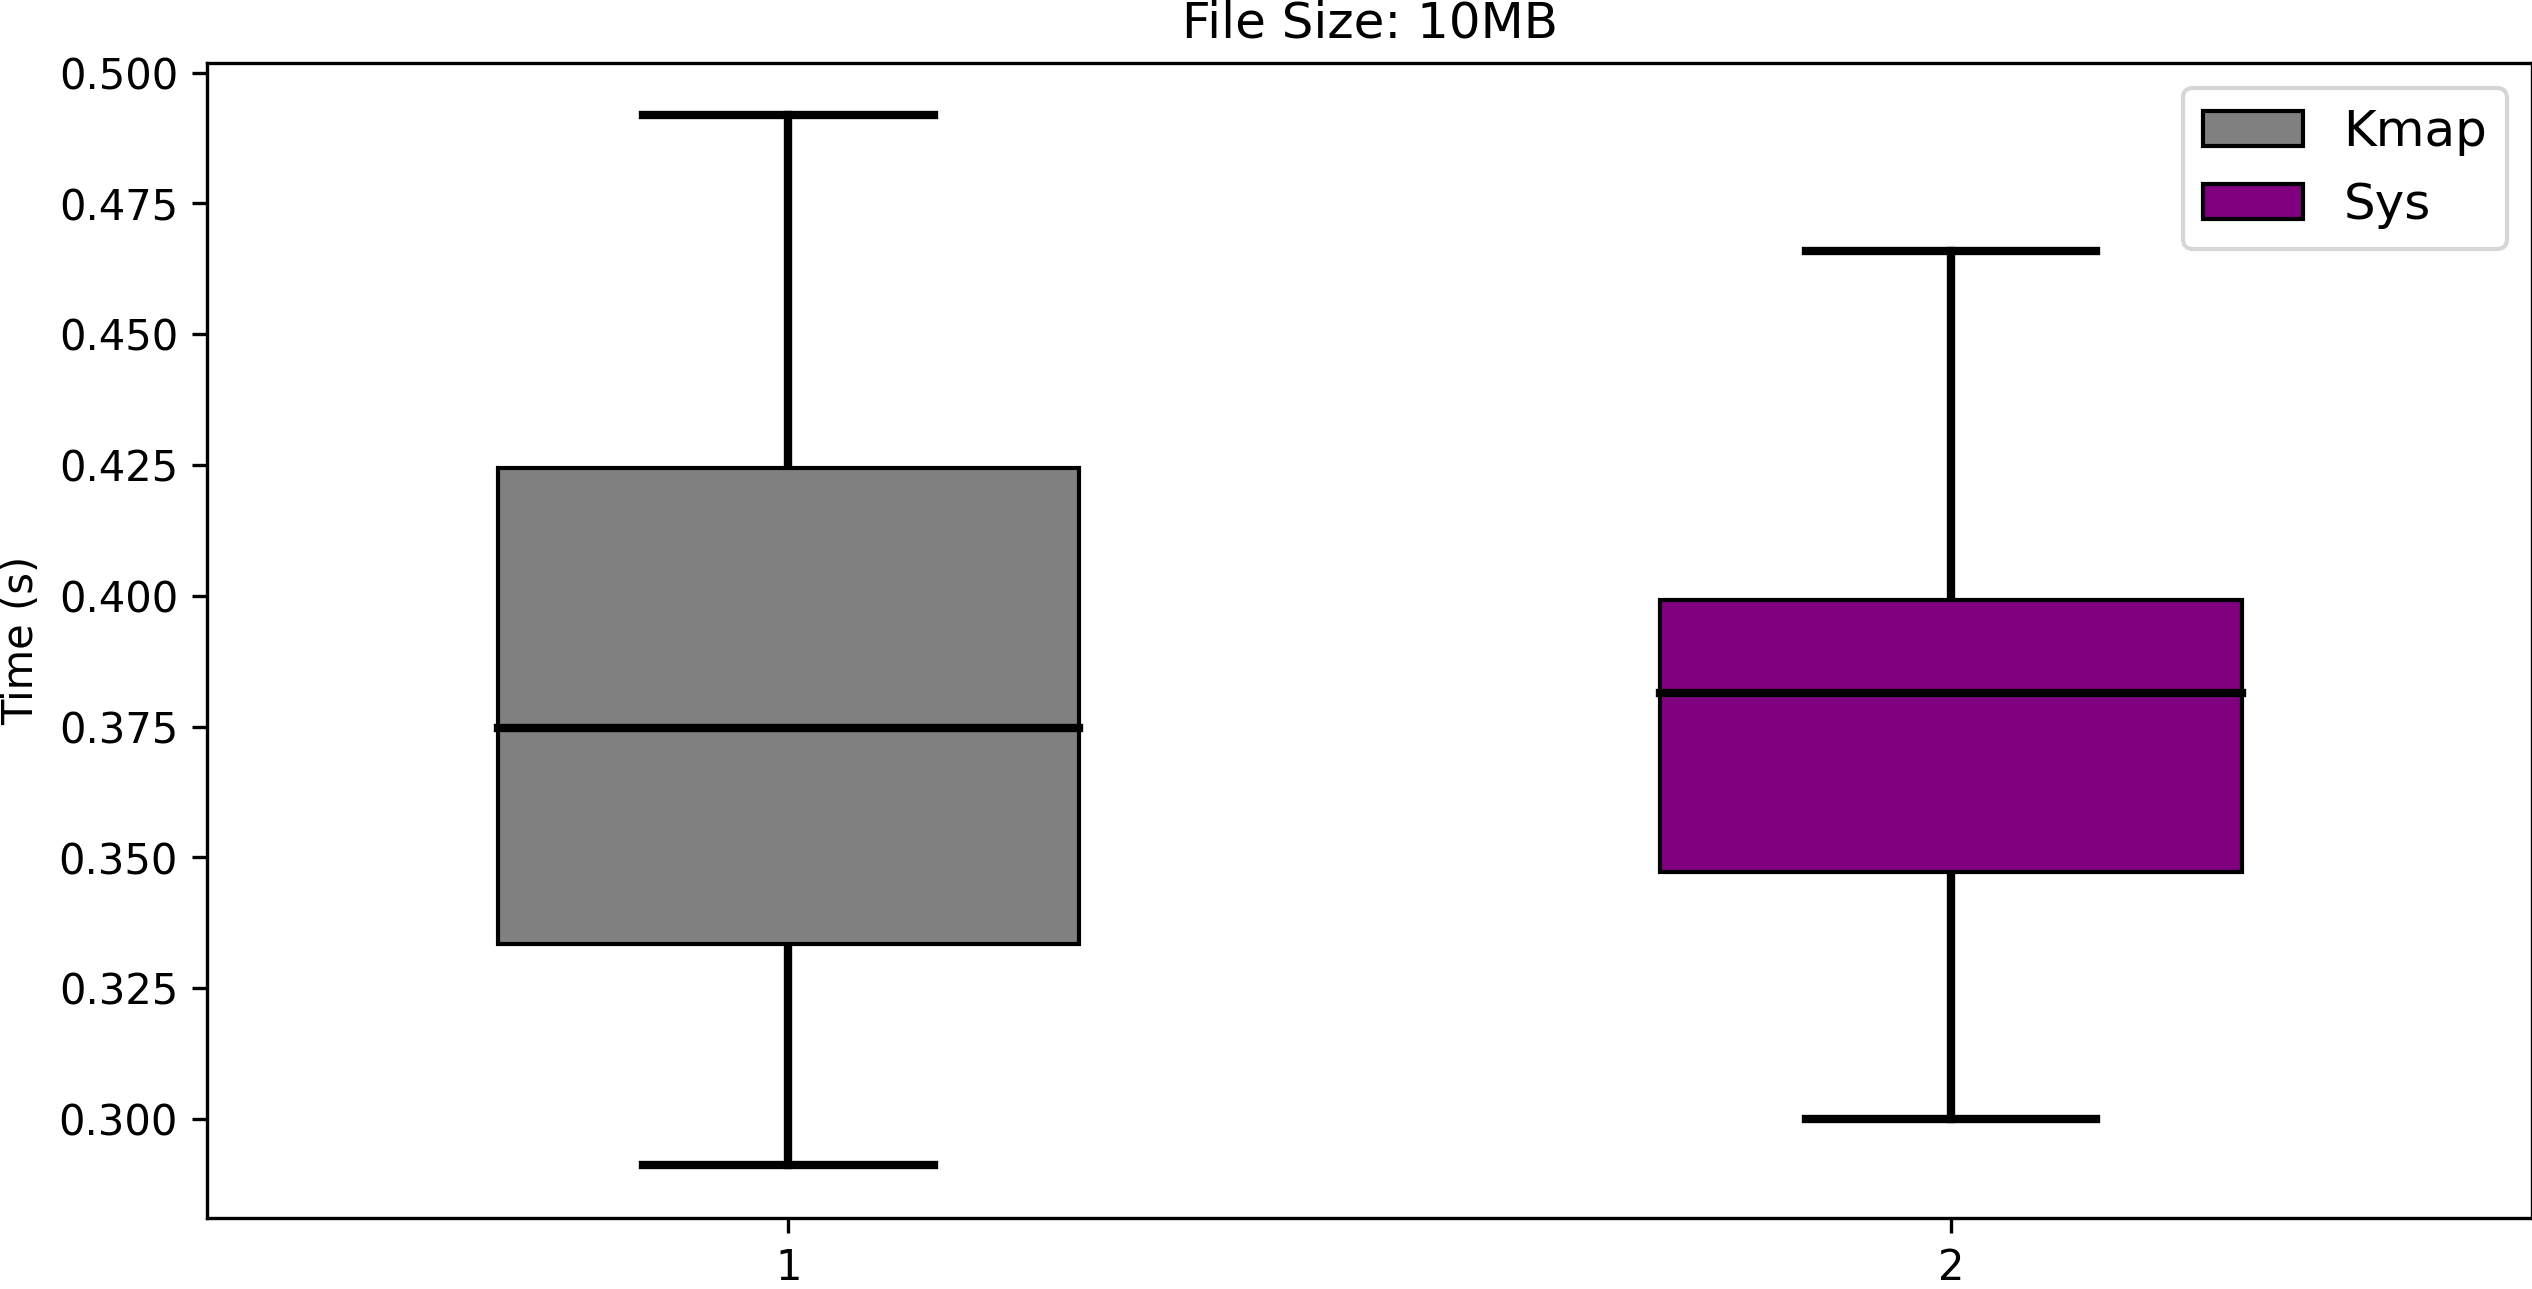
\includegraphics[keepaspectratio=true,width=3in]{figures/evaluation/netload.png}
        \caption{\sysname with Network Under Load}
        \label{fig:netload}
    \end{minipage}%
\end{figure}


\begin{figure*}[!htb]
    \begin{minipage}{0.5\textwidth}
        \centering
        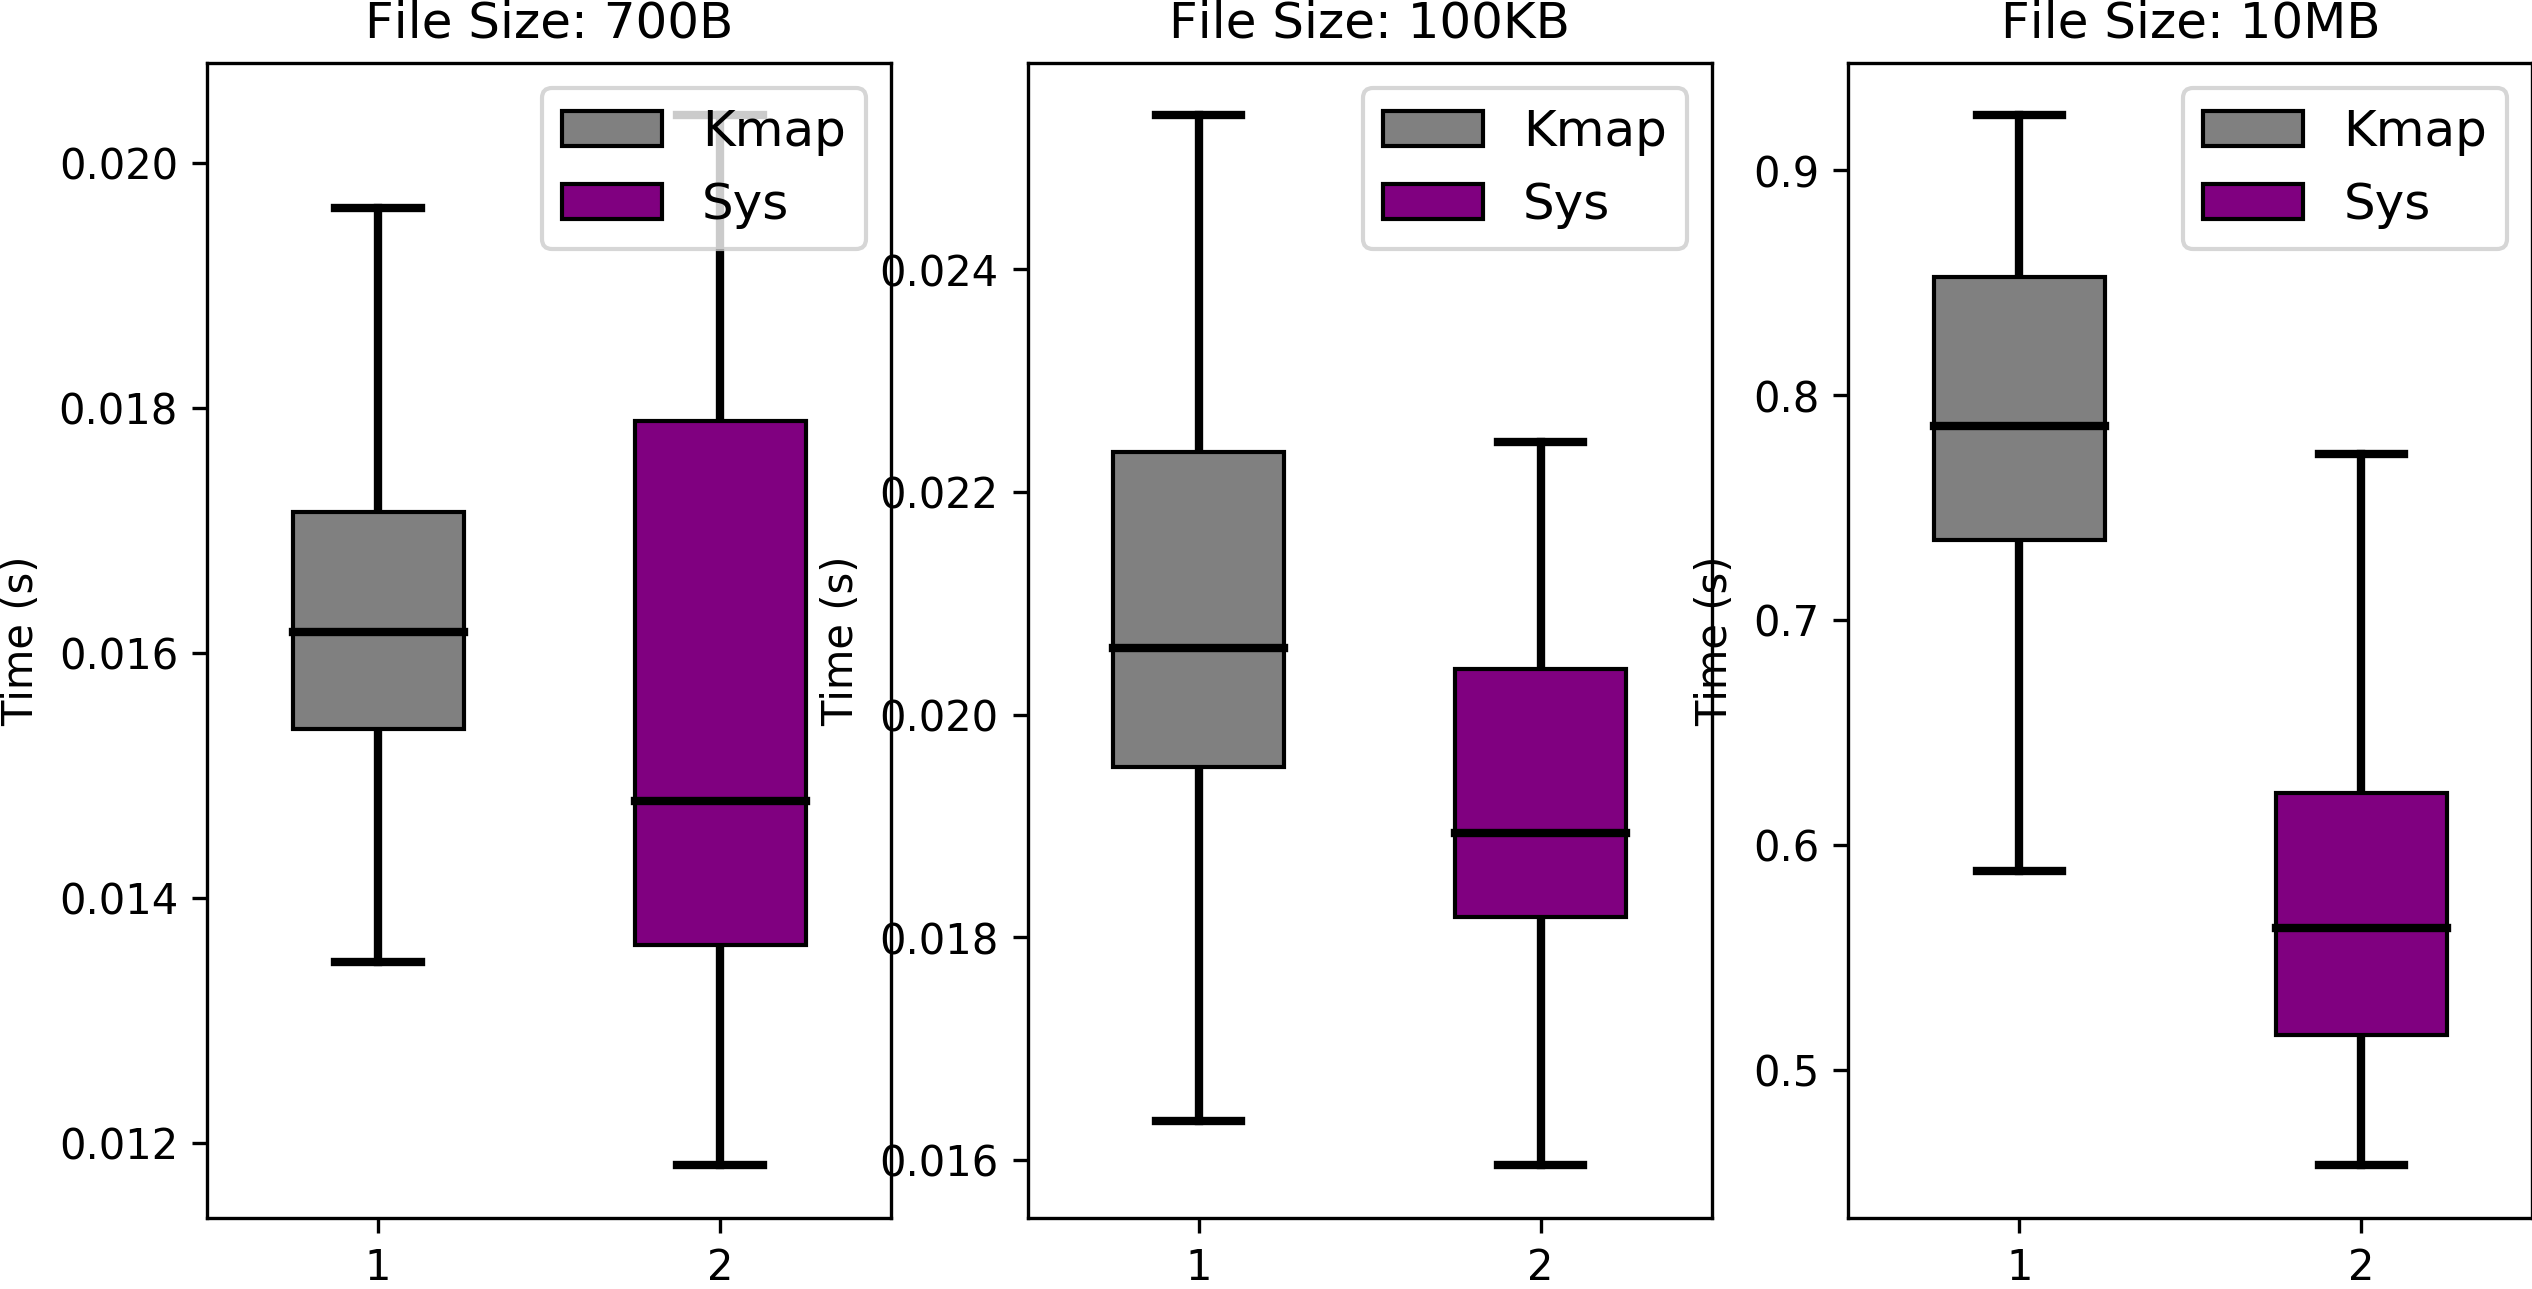
\includegraphics[keepaspectratio=true,width=3in]{figures/evaluation/results.png}
        \caption{Time to Transfer}
        \label{fig:results}
    \end{minipage}%
    \begin{minipage}{0.5\textwidth}
        \centering
        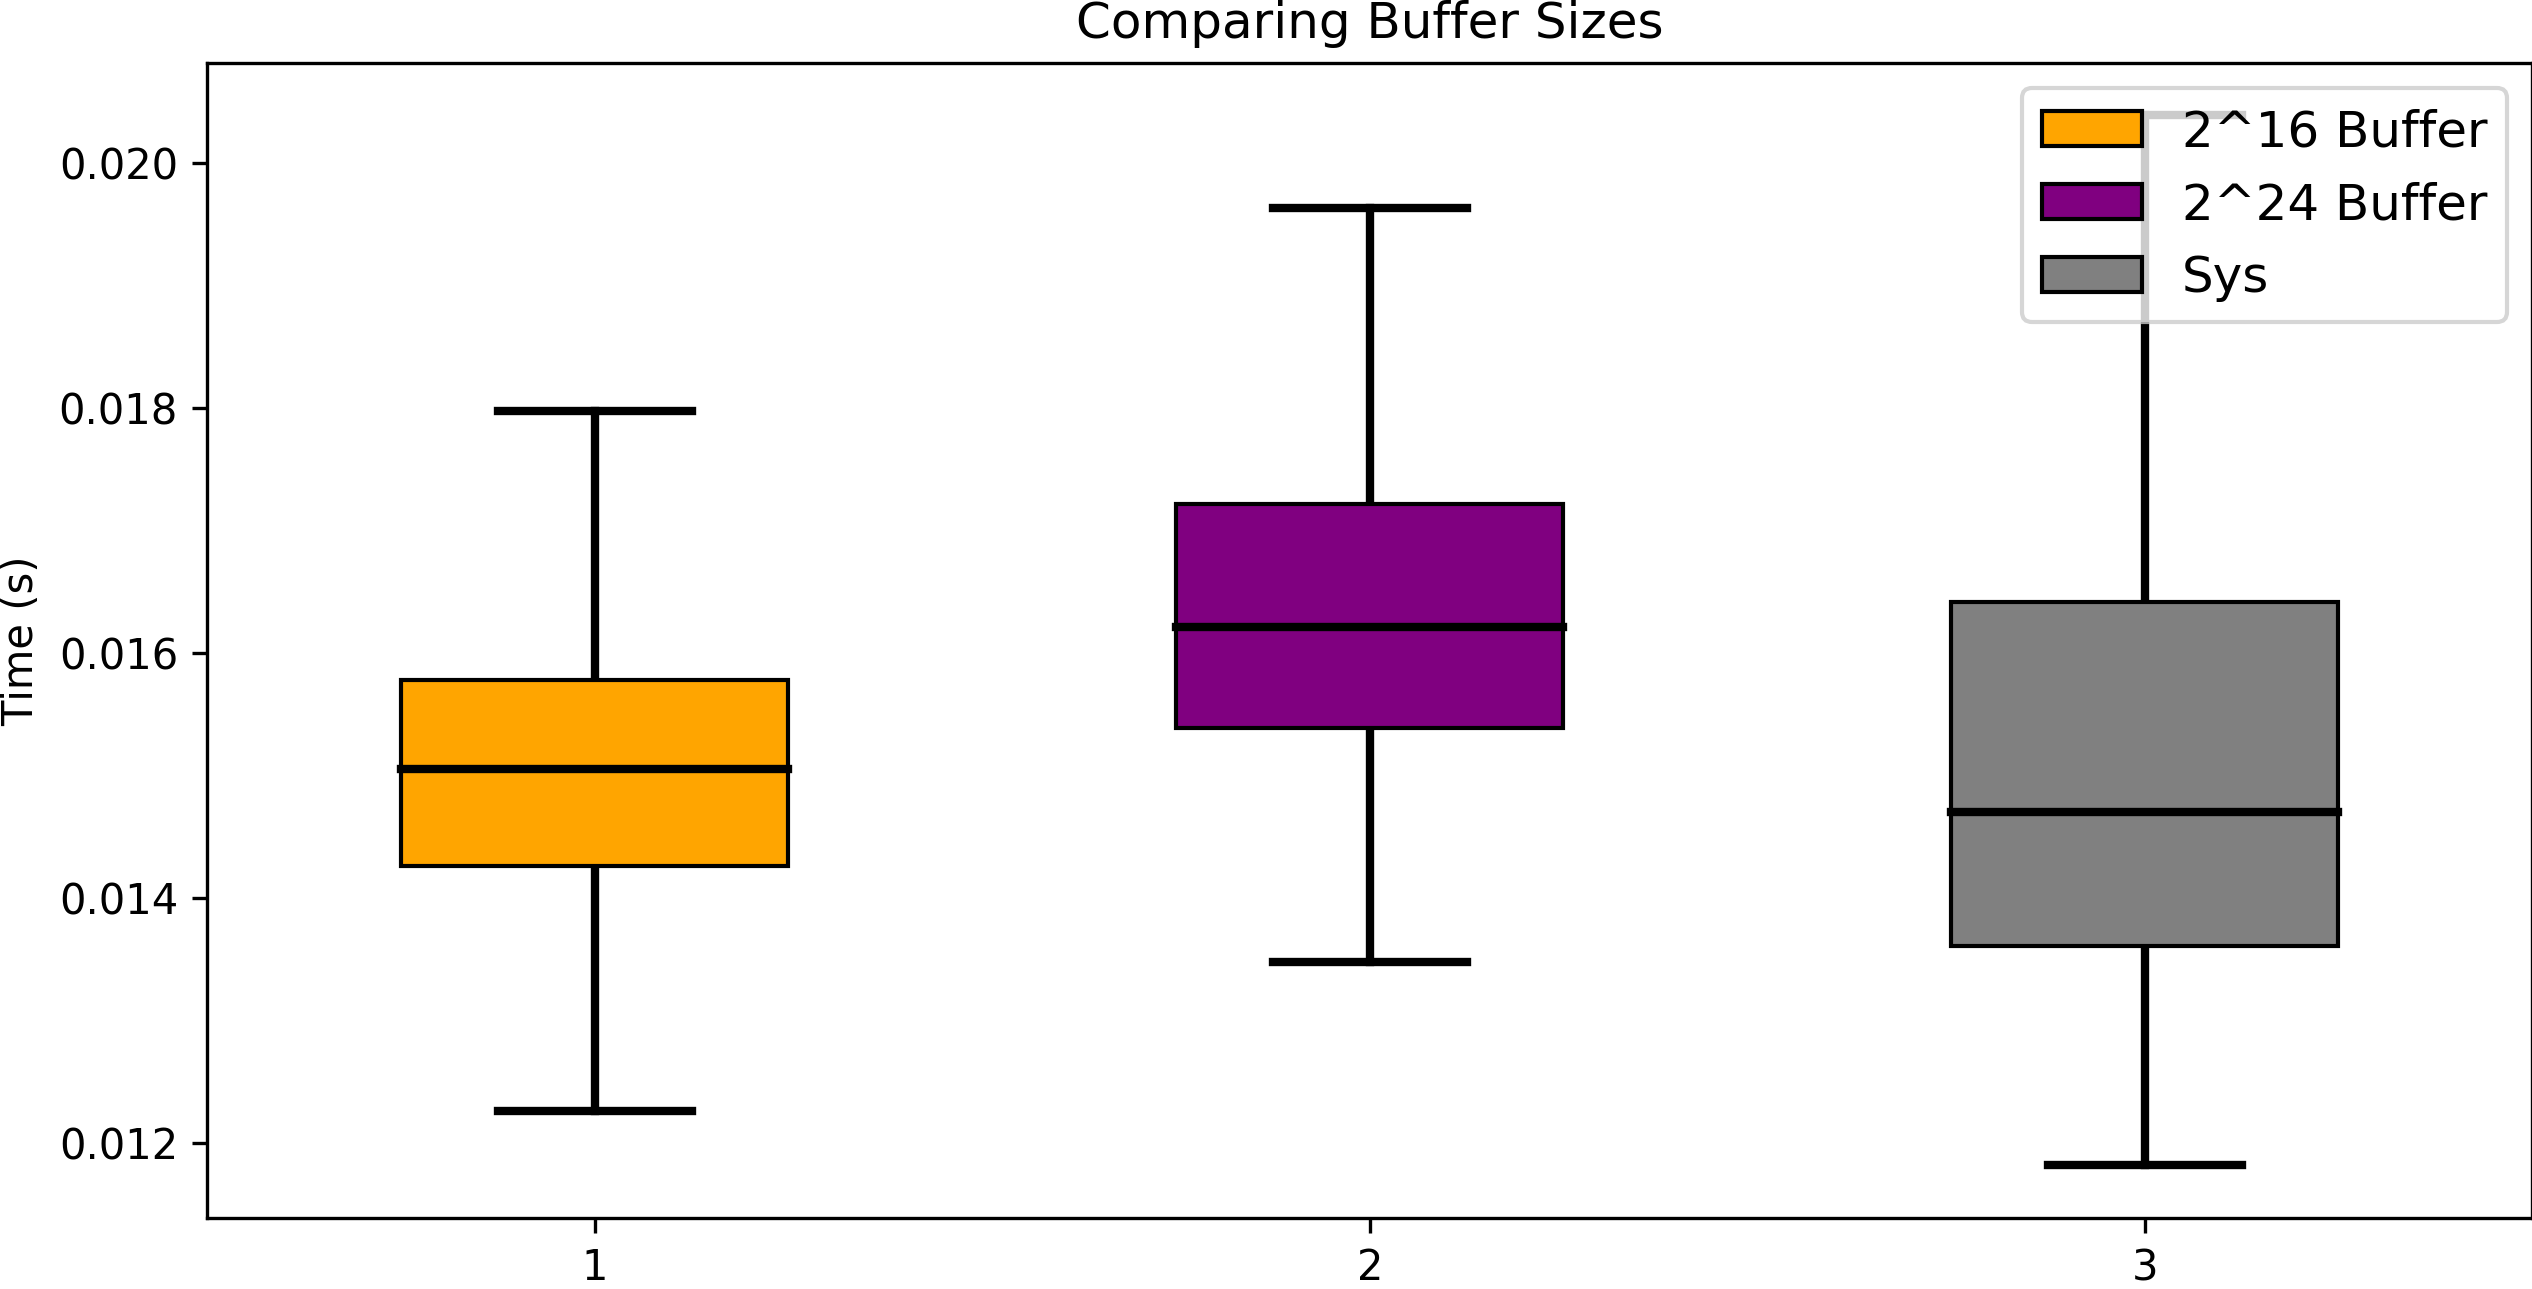
\includegraphics[keepaspectratio=true,width=3in]{figures/evaluation/buf_compare.png}
        \caption{Comparing \sysname Buffer Sizes}
        \label{fig:buf}
    \end{minipage}%
\end{figure*}